\chapter{系统设计}
本章给出了本文设计的非对称半桥反激式变换器系统的性能和设计指标。 首先给出了本文设计的AHB变换器的性能指标,介绍了控制芯片的内部原理图。此外, 为了提高系统的转换效率,分析了反激式变换器的主要损耗,总结了影响系统损耗的主要因素。根据损耗分析的结果,设计了多模式的控制方案,通过系统的带载情况来调节变换器的开关频率和原边的峰值电流值,从而降低系统的损耗,实现系统的整体效率的提升。另外,为了进一步提高系统的转换效率,针对性的提出了两种关键技术,分别用以降低功率管开关损耗和变压器的传导损耗。除此之外,为了降低系统的待机功耗,设计了空载下的突发工作模式。最后为了保证变换器能够稳定的运行,设计了副边反馈网络的二阶补偿结构,并对系统进行了稳定性仿真。


\section{外部电路结构}
本文设计的非对称半桥反激式开关电源变换器的外部电路结构如图所示,包括输入整流回路和反馈回路,为了提高反馈精度,反激回路采用副边反馈结构,通过TL431和光耦模块直接对输出电压进行采样产生误差信号反馈给变换器芯片来为稳定输出电压。

输入回路包括输入整流滤波和片外启动电路两部分,输入整流滤波由四个二极管和电容Cdc组成,将从电网传递进来的交流信号Vac经过整流滤波后转换为直流输入信号Vdc,此输入信号是一个直流的高压,无法直接为变换器芯片进行供电,通过电阻$R_{shunt}$给电容$C_{vdd}$充能给变换器芯片供电,当其超过片内欠压锁定电路的最低电压后芯片开始工作,随着芯片控制高低边功率管的交替通断,辅助绕组能量积攒到一定程度后,二极管D2导通,对电容$C_{vdd}$进行充能,产生变换器输入电压Vdd,代替输入信号Vdc稳定地为变换器芯片电源端进行供电。


\section{系统架构}

\subsection{芯片特点和设计指标}

• 支持宽输入电压范围

• 支持宽输出电压范围

• 高效多模式控制

• 轻载低功耗模式

• 全电压和负载条件下支持零电压导通

\begin{table}[htbp]
    \caption{控制芯片的引脚定义}
    \label{tab:控制芯片的引脚定义}
    \centering
    \belowrulesep=0pt  %防止竖线不连续
    \aboverulesep=0pt  %防止竖线不连续
        \begin{tabular}{c|c|c}
            \toprule
            引脚标号 & 名称 & 功能  \\
            \midrule
            1 & EN   & 使能端                                              \\  \midrule
            2 & VDD  & 变换器芯片内部供电端                                 \\  \midrule
            3 & HSGD & 半桥变换器高边功率管的栅极驱动器,控制高边功率管的通断  \\\midrule  
            4 & LSGD & 半桥变换器高边功率管的栅极驱动器,控制低边功率管的通断  \\\midrule  
            5 & ZCD  & 辅助绕组分压采样端                                    \\  \midrule
            6 & CS   & 变压器原边峰值电流采样端                               \\ \midrule
            7 & VS   & 输入电压分压端                                        \\  \midrule
            8 & GND  & 变换器芯片接地端                                      \\  \midrule
            9 & HB   & 功率管半桥中间节点端                                   \\ 
              
            \bottomrule
        \end{tabular}
\end{table}

\subsection{芯片内部结构}
图~\ref{fig:芯片内部结构图}给出了芯片内部结构架构,该架构包括电源模块、峰值电流控制模块、 退磁检测模块、前沿消隐模块、精确谷底导通模块、谷值锁定模块、前沿消隐(LEB)、退磁时间逐步逼近模块、模式选择模块、逻辑控制模块和驱动等主要模块,每个模块的功能定义如下:

\begin{figure}[htbp] 
    \centering
    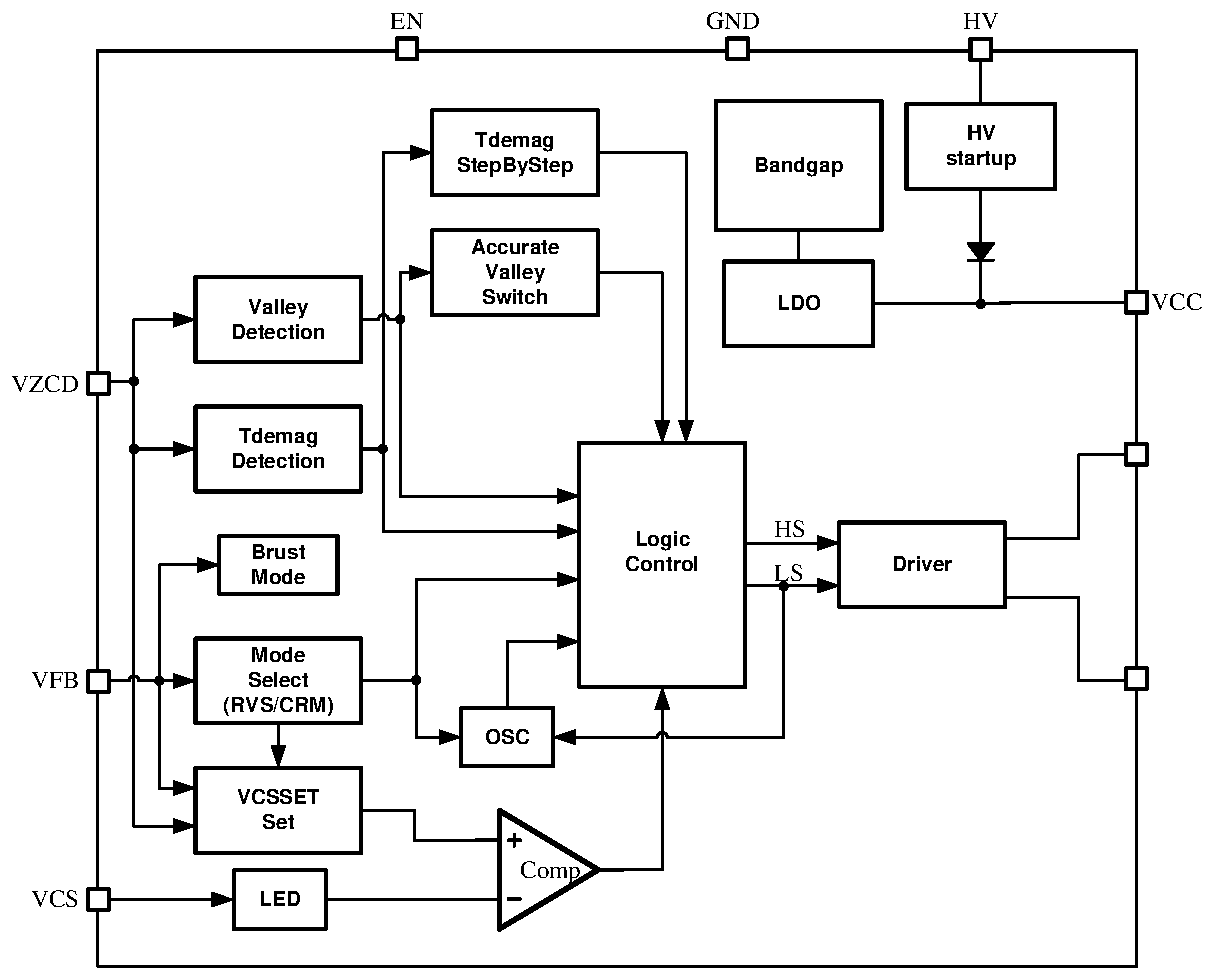
\includegraphics[width=0.8\linewidth]{figures/芯片内部结构图.pdf}
    \caption{芯片内部结构图}
    \label{fig:芯片内部结构图}
\end{figure}

\textbf{电源模块}:电源模块主要包括芯片的欠压锁定电路、带隙基准和降压电路等,该模块的主要作用是为芯片内部各个模块提供稳定的供电电压和各种不受PVT影响的精确偏置电压信号。

\textbf{峰值电流控制模块}:峰值电流控制模块通过对片外副边反馈信号$V_{FB}$和辅助绕组分压信号$V_{ZCD}$进行配置补偿后,产生对应的峰值电流信号Vcspeak,用于和采样电阻上的采样电压信号Vcs进行比较控制高边功率管的导通和关断;该模块的主要功能是为了满足非对称半桥反激式开关电源变换器的宽输出范围下产生相对应的峰值电流信号Vcspeak,防止副边反馈信号$V_{FB}$在不同输出电压相同负载条件下的不匹配,影响后续电路的模式选择控制。

\textbf{退磁检测模块}:退磁检测模块将辅助绕组分压信号$V_{ZCD}$采样后,通过高通滤波电路检测并放大其电压波形上的高频谐振信号并与基准电压比较后,产生对应的输出脉冲来判断变压器原边励磁电感的退磁完成时间,进而控制低边功率管的关断。

\textbf{前沿消隐模块}:功率管导通瞬间会因为系统的寄生参数产生尖峰电流,前沿消隐模块通过屏蔽该尖峰信号以防原边峰值电流控制模块对电流的采样信号出现误判,以此提高电路的稳定性。

\textbf{精确谷底导通模块}:精确谷底导通模块的主要作用是控制低边功率管在半桥节点电压信号$V_{HB}$的谐振谷底处精确导通,模块中的传播延时补偿电路超前判断谐振谷底的到达,基本消除了控制信号经过驱动电路后产生的延时误差,最大限度地降低了功率管的开关损耗,提高了电路传递效率。

\textbf{谷值锁定模块}:谷值锁定模块通过数模混合技术,实现对RVS工作模式下高低边功率管等待时间中半桥节点电压$V_{HB}$谐振谷值数的锁定,主要作用是防止RVS模式时由于输出负载波动导致每周期中谐振谷值不一致,发生跳谷现象,影响电路的稳定性。

\textbf{退磁时间动态校准模块}:退磁时间逐步逼近模块主要作用是控制低边功率管的导通时间,影响变压器中能量对副边输出电容的传递,通过使用可自适应调整斜率的积分器电路来逐步调节低边功率管逐渐对退磁检测模块输出的退磁完成时间进行逼近,实现能量传递的最高效率和副边的零电流导通。

\textbf{模式选择模块}:模式选择模块通过检测副边反馈信号$V_{FB}$和辅助绕组分压信号$V_{ZCD}$来控制变换器IC选择在不同输出电压下和不同输出负载下的控制模式,在空载下使用突发模式降低待机功耗,在轻中载时使用RVS跳谷模式减低开关损耗,在重载时使用CRM模式实现最大能量传递满足负载需要。

\textbf{逻辑控制模块}:逻辑控制模块对模式选择模块的输出信号SE、不同模式的周期导通信号、恒流恒压模式的切换信号等进行逻辑处理,实现输出高低边功率管通断控制信号给驱动模块的作用。

\textbf{驱动模块}:驱动模块用以将逻辑控制模块中所产生的功率管通断控制信号转换为功率管的高低边栅压控制信号,满足功率管所需的大驱动能力和低导通损耗,同时需控制模块的功耗不能过大。

\textbf{保护模块}:保护模块包括过温保护、输出电压欠压和过压保护、芯片供电VDD欠压和过压保护等,其通过检测芯片工作的温度、输出电压值和 VDD 供电电压值的大 小,在芯片温度过高或过低、输出电压不在限制范围和芯片供电不稳定时及时关断芯 片对电路进行保护。

\section{损耗分析}

开关电源系统中的损耗严重影响了系统的转换效率,需要对系统中不同的损耗进行分析和研究。非对称半桥反激式变换器系统中主要的损耗有六种,分别是:功率管开关损耗、功率管导通损耗、变压器的损耗、采样电阻的损耗、输出二极管的损耗和输出电容的损耗。本文将在下面的小节中详细介绍这些损耗的原理和影响因素。

\subsection{功率管开关损耗}

功率管的开关损耗包括开通损耗和关断损耗,分别对应了功率管的导通和关断过程。以开通损耗为例,指的是实际的非理性功率管在导通时,其漏源电压$V-{DS}$并不是立即下降到零,存在一个对应的下降过渡时间;其漏电流$I_{DS}$也不是立即上升到最大值,同样存在一个上升过渡时间,如图~\ref{fig:开关损耗图}所示。在图~\ref{fig:开关损耗图}中可以观察到功率管的$V_{DS}$和$I_{DS}$的波形之间有交叠区域,在这个区域内产生的交越损耗即为开通损耗。关断损耗同理,只是对应的交叠区域出现在功率管的关断时刻。

\begin{figure}[htbp] 
    \centering
    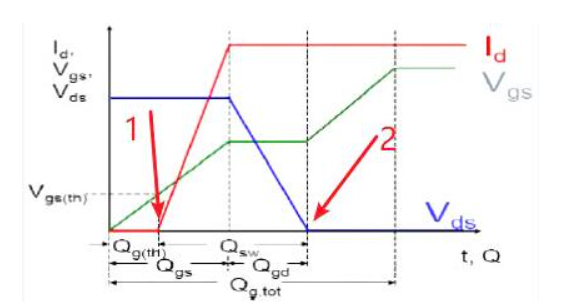
\includegraphics[width=0.6\linewidth]{figures/开关损耗图.png}
    \caption{功率管开通损耗波形图}
    \label{fig:开关损耗图}
\end{figure}

通过文献中的推导,结合图~\ref{fig:开关损耗图}中利用电压和电流的平均化处理可计算得功率管最差情况下的开关损耗,如式\eqref{eq:开关损耗公式}所示:
\begin{equation}
    \label{eq:开关损耗公式}
    P_{sw}=\frac{1}{2} \cdot V_{DS} \cdot I_{DS} \cdot T_{on} \cdot f_{sw} + \frac{1}{2} \cdot V_{DS} \cdot I_{DS} \cdot T_{off} \cdot f_{sw}
\end{equation}
其中,$T_{on}$是功率管的开通时间,$T_{off}$是功率管的关断时间,$f_{sw}$是功率管的开关频率。由式可知,功率管开关损耗主要受到功率管漏源电压、漏电流、开关时间和开关频率的影响。为了降低功率管的开关损耗,可以通过降低开关频率、减小栅极输入电阻减小开关时间、降低峰值电流和实现功率管ZVS条件下的软开关等方式。

\subsection{功率管导通损耗}

功率管的导通损耗是指功率管在完全导通的情况下,无法将其等效为电阻为零的导线,在实际使用的情况下,功率管导通时存在一定的导通电阻$R_{DS,on}$,功率管漏电流流过该电阻后会产生一定的损耗。导通损耗的计算公式如式\eqref{eq:导通损耗公式}所示。
\begin{equation}
    \label{eq:导通损耗公式}
    P_{con} = I_{pri,rms}^2 \cdot R_{DS,on}
\end{equation}
其中,$I_{pri,rms}$是功率管漏电流的有效值。降低功率管导通电阻需要降低反激式变换器系统的原边峰值电流或选用小$R_{DS,on}$的功率管。

\subsection{变压器的损耗}

在开关电源系统中,变压器是用于实现电压转换、原副边电气隔离和能量传递的关键元件,其上产生的损耗也极大的影响了系统的转换效率。变压器的损耗主要包括磁芯损耗(铁损)、绕组损耗(铜损)和漏感损耗等部分。

铁损是由于交变磁场在磁性材料中产生的能量损耗,包括磁芯材料在反复的励磁和退磁过程中都需要克服内部阻力产生的损耗和磁场在磁芯中感应出的涡流通过磁芯电阻产生的损耗。通过斯坦梅茨的铁损模型,铁损的表达式可简化为:
\begin{equation}
    \label{eq:铁损公式}
    P_{core} = K \cdot f_{sw}^\alpha  \cdot B_{max}^\beta \cdot V_{core} 
\end{equation}
其中$K$是损耗系数,$B_{max}$是最大磁场强度,$V_{core}$是磁芯体积。

铜损则是由于电流流过变压器线圈而产生的电阻热损耗。根据铜损模型可推导出铜损的表达式:
\begin{equation}
    \label{eq:铜损公式}
    P_{copper} = I_{rms}^2  \cdot R_{DC} 
\end{equation}
其中$I_{rms}$是流经变压器电流的有效值,$R_{DC}$是变压器线圈的阻抗。

变压器的漏感损耗,指的是由于原边电流对漏感储存的能量无法传递到变压器副边,该部分能量通过功率管或吸收电路被消耗掉产生的损耗,漏感损耗的公式可表达为:
\begin{equation}
    \label{eq:漏感损耗公式}
    P_{lk} = \frac{1}{2}\cdot I_{pri,peak}^2  \cdot f_{sw} 
\end{equation}
其中$I_{pri,peak}$指的是变压原边电感的峰值电流。

\subsection{电流采样电阻损耗}

反激式变换器系统通过使用外接电流采样电阻来检测变压器原边电流,采样电阻上的损耗如式\eqref{eq:导通损耗公式}所示,主要受到采样电阻和原边电流有效值的影响。
\begin{equation}
    \label{eq:采样电阻损耗公式}
    P_{CS} = I_{pri,rms}^2  \cdot R_{CS} 
\end{equation}


\subsection{副边二极管的损耗}

在反激式变换器系统中,副边二极管的损耗占较大比重,式\eqref{eq:二极管损耗公式}表示了副边输出二极管的损耗。
\begin{equation}
    \label{eq:二极管损耗公式}
    P_{diode} = I_{sec,rms} \cdot V_{diode} \cdot D 
\end{equation}
其中$I_{sec,rms}$为副边电流的有效值,$D$为副边输出二极管的导通占空比。

\subsection{输出电容损耗}

开关电源系统中的输出电压由于功率管的开关会产生相应的电压纹波,为了稳定输出电压需要在输出端添加输出电容来滤除输出纹波。但输出电容存在寄生电阻,该电阻可以等效为一个和输出电容串联的$ESR_{out}$电阻,当输出电流流过$ESR_{out}$电阻时会产生电阻热损耗,该损耗的计算公式为:
\begin{equation}
    \label{eq:ESR损耗公式}
    P_{Co} = (I_{sec,rms}^2 - I_{out}^2) \cdot ESR_{out}
\end{equation}

\subsection{损耗总结}

从上问描述的各种损耗的原理可以看出,大部份都与反激式变换器系统的工作电流和开关频率有密切关系,由于反激式变换器一般通过采样原边的电流采样电阻来检测系统的工作电流的大小,因此可以看成这些损耗与系统的原边电感峰值电流相关。由此可以得出,影响系统损耗的两个关键因素为原边的峰值电流和系统的开关频率。

\section{多模式切换}

根据对上文对反激式变换器系统的各种损耗分析可知,为了实现在不同输出电压下和不同输出负载情况下降低系统的损耗,提高系统整体的传递效率,需要根据负载和输出电压的大小自动地调节系统的开关频率和峰值电流。根据文献的研究,反激式变换器系统在重载情况下主导损耗是功率管导通损耗,在轻载条件下主导损耗是功率管开关损耗,因此为了实现全负载范围下的低损耗高效率,需在重载情况时使用CRM模式降低导通损耗,在轻载情况时使用RVS模式降低开关损耗,在空载时使用突发模式实现最小的待机功耗。除此以外,考虑到宽输出范围的影响,不同模式的切换也要受到输出电压的影响。

\begin{figure}[htbp] 
    \centering
    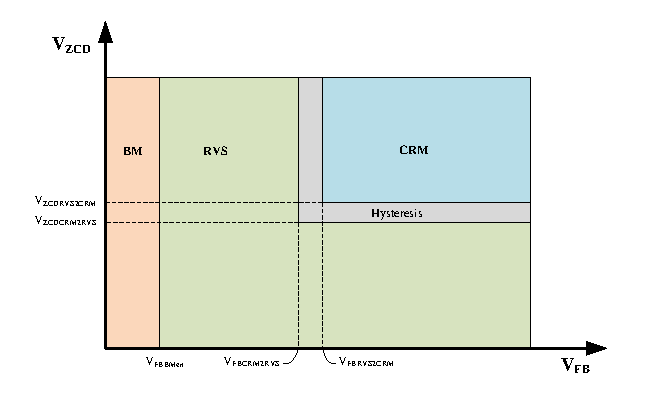
\includegraphics[width=0.8\linewidth]{figures/模式切换1.pdf}
    \caption{多模式切换图}
    \label{fig:模式切换1}
\end{figure}

本文设计了如图~\ref{fig:模式切换1}所示的多模式控制方案,模式切换通过监测引脚FB和引脚ZCD上的电压值来判断输出负载电流和输出电压的大小,一但其超过所设置的不同阈值,模式选择模块控制变换器芯片切换到相应的模式。根据变换器芯片设计,当输出负载电流很小处于极轻载或空载情况时,$V_{FB}$小于对应的参考电压$V_{FBBMen}$,此时芯片被设定为突发工作模式;当输出负载电流逐渐增大进入轻载情况,$V_{FB}$同样随着输出负载电流的增大而增大,且其未大于$V_{FBRVS2CRM}$时,芯片工作在RVS模式中,RVS工作模式是非对称半桥反激式开关电源所特有的一种新型工作模式,能最大化地同时降低高低边功率管的开关损耗;当输出负载电流继续增大,进入重载情况后,$V_{FB}$此时大于$V_{FBRVS2CRM}$,芯片被从RVS工作模式切换为CRM工作模式,在不影响变压器中储能转换的情况下,实现最大的开关频率,最大限度地降低功率管导通损耗并为副边传递能量,维持输出电压在重载下的稳定性。为了防止模式切换时的不稳定性问题,避免芯片在两个模式中来回切换,针对性的设置了CRM模式和RVS模式之间的迟滞区间,当负载电流从重载向轻载切换时,$V_{FB}$则需要小于$V_{FBCRM2RVS}$时,才能由CRM模式切换为RVS模式。由文献可知,AHB反激式变换器系统在轻载时使用CRM模式无法达到最大的能量传递效率,因此输出电压同时制约着不同模式的切换,通过辅助绕组的分压引脚$V_{ZCD}$监测输出电压大小,根据计算和测试,选择输出电压大于15V后才允许芯片从RVS模式切换为CRM模式。为了避免模式之间的频繁切换引起的电路振荡,$V_{ZCD}$同样设置有两个偏置电压$V_{FBRVS2CRM}$和$V_{FBCRM2RVS}$作为迟滞区间。

\begin{figure}[htbp] 
    \centering
    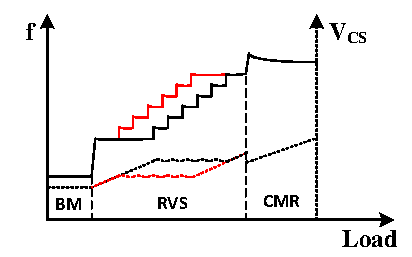
\includegraphics[width=0.8\linewidth]{figures/模式切换2.pdf}
    \caption{多模式频率变化图}
    \label{fig:模式切换2}
\end{figure}

不同的模式影响着功率管的开关频率和峰值电流变化,如图~\ref{fig:模式切换2}所示。

在突发模式时,功率管开关频率和峰值电流都被设定为最小值,通过控制系统间歇性地工作,关断芯片内部除供电模块的所有的控制模块,降低系统的待机功耗;

在RVS工作模式时,功率管开关频率随着输出负载电流的增大呈阶梯式波动,这是由于RVS工作模式为了减小开关损耗,只在高低边功率管中间节点电压$V_{FB}$谐振波谷的谷底处触发导通信号,开始新的周期;为了防止开关频率和峰值电流共同变化导致变换器系统的相位降低引起的稳定性问题,变压器原边电感的峰值电流则不随开关频率的变化产生剧烈波动,通过谷底锁定模块将其维持在一个稳定的区间,以适应输出功率的变化。

在CRM工作模式时,功率管开关频率随着输出负载电流的增大提高到当前变换器系统LC谐振腔允许的最大开关频率;变压器原边电感的峰值电流随输出负载电流的增大而增大,以满足最大工作频率下输出功率的需要。CRM工作模式的工作频率达到最大值后有缓慢减小的趋势,这是由于低边功率管因为LC谐振腔的谐振周期限制了退磁时间的大小,而高边功率管的导通时间随着峰值电流的增大而增大,导致开关周期相应变长,开关频率缓慢降低。

\subsection{CRM工作模式}

\subsection{RVS工作模式}

\begin{figure}[htbp] 
    \centering
    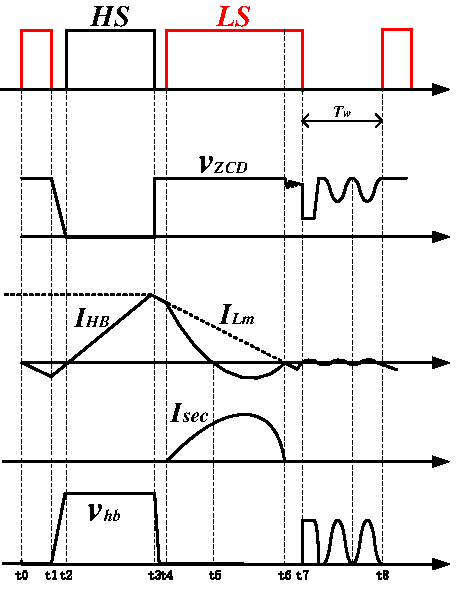
\includegraphics[width=0.6\linewidth]{figures/RVS波形图.pdf}
    \caption{RVS工作模式波形图}
    \label{fig:RVS波形图}
\end{figure}

RVS工作模式是针对非对称半桥反激式开关电源设计的一种新型的DCM操作模式,旨在轻载工况下消除高低边功率管的输出损耗。由于非对称半桥反激式变换器拓扑结构初级测和LLC型开关电源相同,存在谐振电容Cr和变压器漏感Lr组成的谐振腔,因此当控制器处于DCM控制模式时,高低边功率管都关闭的等待时间内产生谐振现象,如图~\ref{fig:RVS波形图}中Tw时间。因此无法在等待时间内利用逆向电感电流将高低边功率管中间节点电压$V_{HB}$充电到等于输入电压$V_{in}$,高边功率管存在较大的源漏电压差$V_{DS}(V_{DS}=V_{in}-V_{HB})$,故在非对称半桥反激式系统中使用传统的DCM控制方式导通高边功率管会产生巨大的开关损耗,降低电路的能量传递效率,因此非对称半桥反激式系统中一般使用边界导通(BCM)模式,BCM工作模式在重载时具有最佳的效率,在轻载时同样存在一定的问题,如能量传递延后和能量传递出现双脉冲等情况。根据文献的研究,提出了新型的谐振谷值开关工作(RVS)模式。

此控制方式巧妙地在开启高边功率管前,提前打开底边功率管一定时间,产生逆向的电感电流为$V_{HB}$节点进行充电,合理规划死区时间即可将$V_{HB}$节点电压充电到等于$V_{in}$,此时再打开高边功率管对变压器原边电感进行励磁储能,极大的降低开关损耗和能量传递效率,具体波形图如图~\ref{fig:RVS波形图}所示。同时考虑到等待时间内$V_{HB}$的谐振情况,通过精确谷底导通模块控制低边功率管在$V_{HB}$电压谐振谷底处导通,抑制低边功率管引入的不必要的开关损耗。

\section{恒流恒压控制模式设计}
反激式变换器系统的控制模式主要分为恒流模式(CC)和恒压模式(CV)。当输出电压还升高到额定电压时,此时变换器芯片工作在恒流模式,输出端以恒定的输出电流为输出电容和输出负载充电,直至输出电压达到额定电压转为恒压模式,维持输出电压的稳定。
\subsection{恒流控制模式}

下面分析输出电流和原边电感电流之间的关系,每个半桥开关周期的输入功率取决于谐振电容Cr上的平均电压$V_{cr\_avg}$,该电压在高边功率管HS导通期间由原边电感电流$I_{HB}$充电。输入功率和输出功率的表达式分别如式\eqref{eq:Pin_1}和\eqref{eq:Pout_1} :
\begin{equation}
    \label{eq:Pin_1}
    P_{in}=\frac{1}{2} \cdot V_{cr\_avg} \cdot (I_{hbpos}+I_{hbneg})
\end{equation}
\begin{equation}
    \label{eq:Pout_1}
    P_{out}=V_o \cdot I_o
\end{equation}
其中$I_{hbpos}$和$I_{hbneg}$分别是变压器原边电感电流的正向电流峰值和负向电流峰值。

假设变压器原边和副边线圈的能量在理想情况下完全传递即$P_{in}=P_{out}$,由式\eqref{eq:Vcr_1}、\eqref{eq:Pin_1}和\eqref{eq:Pout_1}可以得到输出电流的表达式,如式\eqref{eq:Io_1}所示:
\begin{equation}
    \label{eq:Io_1}
    I_o=\frac{N}{2}\cdot(I_{hbpos} + I_{hbneg})
\end{equation}

根据式\eqref{eq:Io_1}可知输出电流完全取决于原边励磁电感中的正负峰值电流。因此,只需要确定了原边励磁电感中的正负峰值电流即可实现恒定的输出电流。

\subsection{恒压控制模式}

当输出电压达到电路设计的额定电压时,变换器芯片的控制模式由恒流模式转换为恒压模式,控制输出电压稳定在额定电压附近。反激式变换器的输入功率和输出功率的公式还可表达为:
\begin{equation}
    \label{eq:Pin_2}
    P_{in} = \frac{E_P}{T}=\frac{1}{2} \cdot L_m \cdot I_{hbpos} \cdot \frac{1}{T}
\end{equation}
\begin{equation}
    \label{eq:Pout_2}
    P_{out} = \frac{V_o^2}{R_L} 
\end{equation}
其中,$E_P$是励磁电感的励磁能量,$T$是开关周期时间,$R_L$是输出负载电阻。

同样假设输入功率等于输出功率,忽略变压器的损耗,由式\eqref{eq:Pin_2}和\eqref{eq:Pout_2}可以得到输出电压的表达式,如式\eqref{eq:Vo_1}所示:
\begin{equation}
    \label{eq:Vo_1}
    V_o = I_{hbpos} \cdot \sqrt{\frac{L_m R_L}{2T}}
\end{equation}
由该式可见得,当输出负载电阻发生变化,而原边电感峰值电流和开关周期未发生时,输出电压会随着负载电阻的变化而变化。输出电压变化后,经过分压电阻分压后输入副边反馈环路中,通过TL431和光耦模块产生电压$V_{FB}$通过副边反馈引脚$FB$输入芯片内,控制系统在不同工作模式下的峰值电流和开关频率大小。在RVS工作模式时,保持峰值电流的相对稳定,通过改变开关频率的大小逐渐调节输出电压恢复其额定电压;在CRM工作模式时,保持开关频率的恒定,通过逐渐改变峰值电流的大小维持输出电压的恒压控制。


\section{关键技术}

\subsection{退磁时间动态校准技术}

AHB反激式变换器系统通过导通高边功率管对变压器原边励磁电感和谐振电容进行储能,导通低边功率管对励磁电感和LC谐振腔中的能量传递到变压器副边的输出电容中,高低边功率管的交替导通实现在不同负载情况下系统的宽范围输出电压稳定。不同于高边功率管的导通时间由峰值电流决定,低边功率管的导通时间设置目前仍未得到广泛探索,低边功率管导通时间过长或过短都存在一定的问题。

过长的低边功率管导通时间实现了变压器副边二极管的ZCS关断,但在高输出电压的情况下会增大不必要的导通损耗,且会继续LC谐振腔内的能量,影响下一周期副边二极管的正向偏置,产生可靠性问题;过短的低边功率管导通时间既可能造成副边的电流纹波增大,无法实现副边二极管ZCS关断,又未能将励磁能量完全传递到副边输出电容,影响系统传递效率。因此无论是重载工况下的CRM工作模式还是轻载工况时的RVS工作模式,都要求低边功率管的最佳导通时间是导通后在励磁电感退磁完成时刻关断功率管。

由文献可知,如~\ref{fig:RVS波形图}中的t6时刻,当变压器原边电感电流$I_{Lm}$和$I_{Lr}$相等时,变压器副边电流$I_{sec}$同时降低为0,原边励磁电感退磁完成,此时副边二极管的寄生电容$C_{pj}$迅速放电且与变压器漏感发生高频谐振,谐振频率公式如\eqref{eq:ZCD谐振公式}所示。

\begin{equation}
    \label{eq:ZCD谐振公式}
    f_{hp} = \frac{1}{2\pi \sqrt{L_r * C_{pj}/N^2}}
\end{equation}

其中 
\begin{equation}
    \label{eq:变压器匝比}
    N=\frac{N_P}{N_S}
\end{equation}

此高频谐振现象可以在ZCD引脚中观察到,故通过对ZCD引脚电压$V_{ZCD}$进行采样处理后,即可得到励磁电感退磁完成信号LST\_e。

包含有退磁时间动态自校准模块的非对称半桥反激式变换器系统的简单框图如图~\ref{fig:退磁时间1}所示,辅助绕组$N_A$上的绕组电压由电阻$R_1$和$R_2$分压后通过ZCD引脚输入变换器芯片中,经采样保持电路处理后输入给退磁时间动态校准模块,最终该模块输出低边功率管的导通时间信号$T_{Q2}$。在模块中不仅需要检测出上文所提到的ZCD引脚上的高频谐振现象,同时输出负载电流波动还会导致的励磁电感退磁完成时刻不固定的问题,针对此问题该模块还新颖的设计了动态自校准的方案,避免低边功率管导通时间随着退磁完成时刻的波动而剧烈变化,引入不必要的人为电路噪声和不稳定性问题,通过一系列电路设计,使得低边功率管导通时间在退磁完成时刻波动后,随着周期的推进,导通时间动态地逐步逼近到退磁完成时刻,实现对退磁完成时刻的精确校准,既满足副边电流ZCS的关断又达到励磁电感能量最佳传递效率。

\begin{figure}[htbp] 
    \centering
    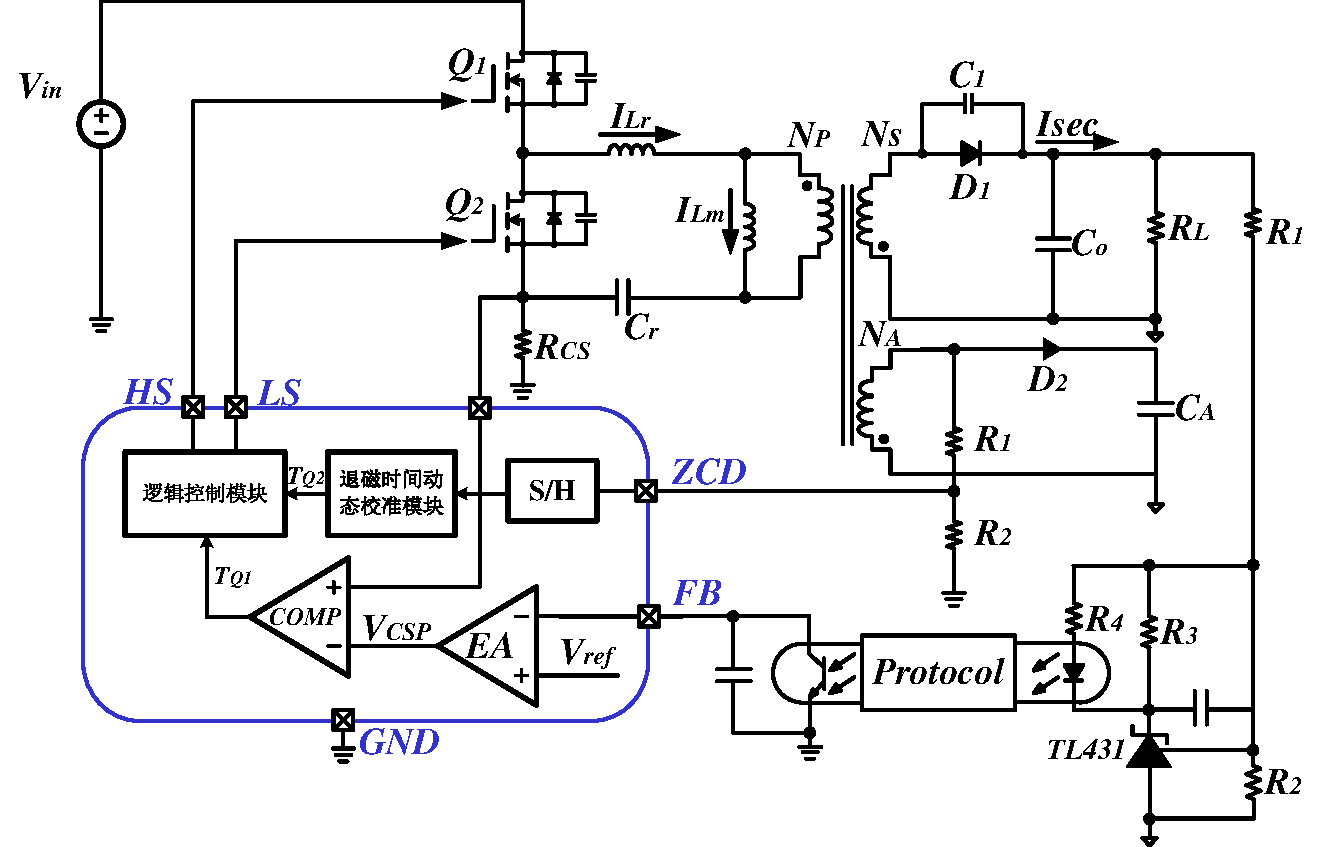
\includegraphics[width=0.8\linewidth]{figures/退磁时间动态校准图.pdf}
    \caption{退磁时间动态校准技术框图}
    \label{fig:退磁时间1}
\end{figure}


\subsection{精确谷底导通技术}
当AHB变换器芯片处于RVS工作模式时,存在如图~\ref{fig:RVS波形图}所示的$T_w$等待时间,此时高低边功率管都关断,此时原边电感不给副边传递能量,原边电感和功率管寄生电容发生谐振现象,功率管半桥节点电压$V_{HB}$自由振荡。为了发挥在RVS工作模式的最佳优势,未采用传统反激式变换器中准谐振模式使用的方案,仅通过比较器将谐振信号和参考电压比较后判断到波谷的位置,即导通功率管的方案。而是新颖地设计了精确谷底导通技术,控制低边功率管在$V_{HB}$电压谐振谷底处精确导通,最大程度地减小低边功率管的开关损耗。

该技术电路解决了两个困难点,一方面是精确监测$V_{HB}$的谐振电压谷底,产生对应谷底信号参与后续逻辑控制;另一方面是解决驱动电路导致的信号延时问题,防止控制功率管的栅极驱动信号比逻辑控制信号更晚产生导致的实际低边功率管滞后于$V_{HB}$的谐振谷底处导通,产生不必要的开关损耗。

图~\ref{fig:RVS波形图}中等待时间$T_w$内显示了一个开关周期内$V_{HB}$信号自由谐振的波形;但因为$V_{HB}$电压过高无法直接输入变换器芯片内进行采样处理,且该谐振现象同时反映在辅助绕组分压引脚ZCD上,如图~\ref{fig:RVS波形图}中$V_{ZCD}$信号的波形,因此将辅助绕组电感电压通过电阻分压后产生的$V_{ZCD}$信号输入变换器芯片内的进行采样处理。

包含有精确谷底导通技术模块的AHB反激式变换器系统的简单框图如图~\ref{fig:精确谷底导通技术框图}所示,LS和LSGD分别是逻辑控制电路和驱动电路针对低边功率管产生的逻辑控制信号和栅极驱动信号,引脚ZCD将带有谐振信息的电压波形输入变换器芯片后经过一个低通滤波器(low pass filter)电路滤波后输入到精确谷底导通模块中。副边反馈信号也通过FB引脚输入到片内谷值锁定电路中进行处理,产生一个RVS工作模式下适应变换器系统负载工况下的等待时间$T_w$,同样输入到精确谷底导通模块中。同时为了解决驱动电路的延时逻辑控制信号问题,将输出的低边功率管栅极驱动信号输入到该模块中。经过该模块内一系列电路的处理,最终输出一个受到谷值锁定电路锁定时间限制的,超前于$V_{HB}$谐振谷谷底一个驱动延时的CLK信号,保证低边功率管在$V_{HB}$的谐振谷最低处导通,最小化功率管开关损耗,提高了电路传递效率。同时为了应对不同工况下的变化,该模块对CLK信号同样进行动态控制,通过补偿环路将其逐渐逼近到最佳位置。



\begin{figure}[htbp] 
    \centering
    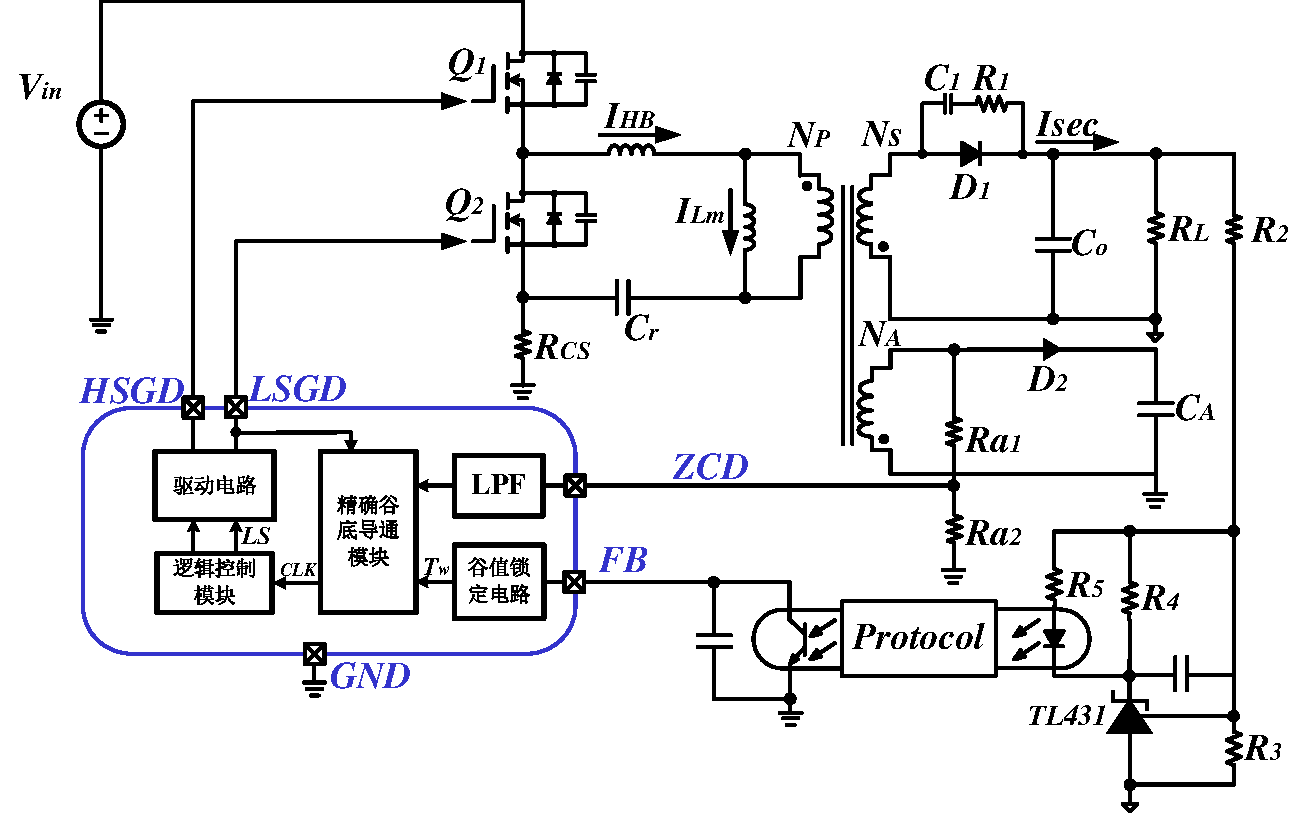
\includegraphics[width=0.8\linewidth]{figures/精确谷底导通技术框图.pdf}
    \caption{精确谷底导通技术框图}
    \label{fig:精确谷底导通技术框图}
\end{figure}



\section{小结}

本章对变换器芯片的整体进行了系统性的描述,首先分析了芯片的外围电路的设计,简单介绍了外部交流转直流和对芯片启动与供电的过程;其次介绍了芯片的主要指标和内部电路的具体组成部分;之后对反激式变换器系统的几种损耗进行了具体的分析,得出降低损耗的方法;紧接着介绍了芯片在不同负载情况下多种工作模式的切换过程,分析了在不同模式下峰值电流和开关频率的关系;然后介绍了芯片的恒流和恒压两种控制模式的具体工作原理和环路构成;最后针对如何进一步提高对AHB反激式拓扑的转换效率,提出了两种新颖的关键技术,简单介绍了它们的使用优势和工作过程,具体电路介绍将在后续章节内进行详细分析。


